\documentclass{article}
\usepackage{amsmath, amssymb, amssymb}
\usepackage{tikz}
\usepackage{tikz-3dplot}

\begin{document}
\begin{center}
    \begin{LARGE}
        \textbf{Introduction to Electromagnetism}
    \end{LARGE}
\end{center}

\section{Coulomb's Law}

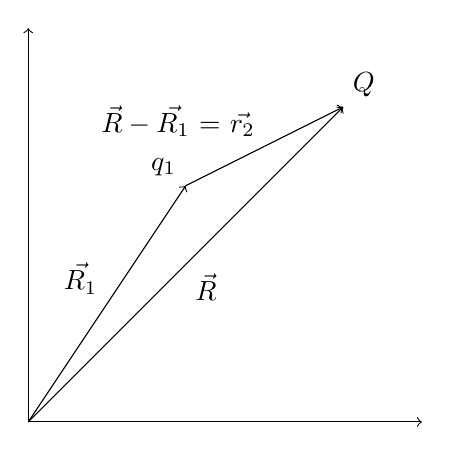
\begin{tikzpicture}
    \draw[->] [black] (0,0) -- (0, 5);
    \draw[->] [black] (0,0) -- (5, 0);
    \draw[black] (0,0) -- (2,2) node[anchor=north west] {$\vec{R}$};
    \draw[->] [black] (2,2) -- (4,4) node[anchor=south west] {$Q$};
    \draw[black] (0, 0) -- (1,1.5) node[anchor=south east] {$\vec{R_1}$};
    \draw[black, ->] (1,1.5) -- (2,3) node[anchor=south east] {$q_1$};
    \draw[black] (2,3) -- (3,3.5) node[anchor=south east] {$\vec{R} - \vec{R_1}$ = $\vec{r_2}$};
    \draw[->] [black] (3,3.5) -- (4,4);

\end{tikzpicture}
the force on $Q$ due to $q_1$ is given by:
$$\vec{F_1} = \frac{1}{4\pi\epsilon_0} \frac{q_1Q}{r_1^2} \hat{r_1}$$

If there was another charge $q_2$ at $\vec{r_2}$: 

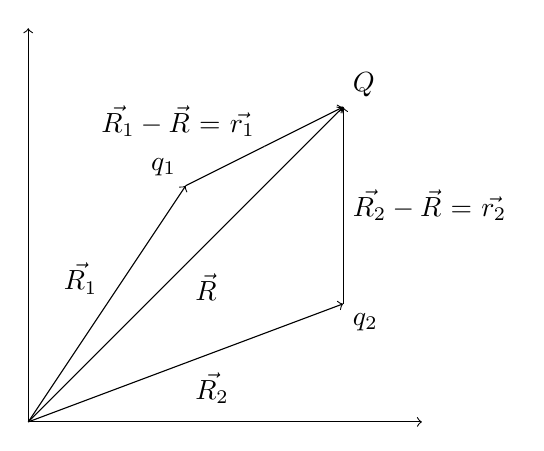
\begin{tikzpicture}
    \draw[->] [black] (0,0) -- (0, 5);
    \draw[->] [black] (0,0) -- (5, 0);
    \draw[black] (0,0) -- (2,2) node[anchor=north west] {$\vec{R}$};
    \draw[->] [black] (2,2) -- (4,4) node[anchor=south west] {$Q$};
    \draw[black] (0, 0) -- (1,1.5) node[anchor=south east] {$\vec{R_1}$};
    \draw[black, ->] (1,1.5) -- (2,3) node[anchor=south east] {$q_1$};
    \draw[black] (2,3) -- (3,3.5) node[anchor=south east] {$\vec{R_1} - \vec{R}$ = $\vec{r_1}$};
    \draw[->] [black] (3,3.5) -- (4,4);
    \draw[black] (0, 0) -- (2,0.75) node[anchor=north west] {$\vec{R_2}$};
    \draw[black, ->] (2,0.75) -- (4,1.5) node[anchor=north west] {$q_2$};
    \draw[black] (4,1.5) -- (4,2.75) node[anchor=west] {$\vec{R_2} - \vec{R}$ = $\vec{r_2}$};
    \draw[->] [black] (4,2.75) -- (4,4);

\end{tikzpicture}

The force on $Q$ due to $q_2$ is given by:
$$\vec{F_2} = \frac{1}{4\pi\epsilon_0} \frac{q_2Q}{r_2^2} \hat{r_2}$$

And the net charge on $Q$ is given by:
$$\vec{F} = \vec{F_1} + \vec{F_2}$$
$$\vec{F} = \frac{1}{4\pi\epsilon_0} \frac{q_1Q}{r_1^2} \hat{r_1} + \frac{1}{4\pi\epsilon_0} \frac{q_2Q}{r_2^2} \hat{r_2}$$

If there were $n$ charges, the net force on $Q$ would be:
$$\vec{F} = \sum_{i=1}^n \frac{1}{4\pi\epsilon_0} \frac{q_iQ}{r_i^2} \hat{r_i}$$
$$\vec{F} = Q \sum_{i=1}^n \frac{1}{4\pi\epsilon_0} \frac{q_i}{r_i^2} \hat{r_i}$$

where $\sum_{i=1}^n \frac{1}{4\pi\epsilon_0} \frac{q_i}{r_i^2} \hat{r_i}$ is the electric field $\vec{E}$ at $\vec{R}$ due to the $n$ charges.

\textbf{Field}: A value, vector or tensor, that is defined for every point in space and time.\\[1pt] 

\section{Vector Calculus}

\paragraph{Vectors} A vector is a quantity that is said to transform like a displacement.\\[1pt]

\subsection*{Operations on Vectors}
\begin{itemize}
    \item \textbf{Addition}: $\vec{A} + \vec{B} = \vec{C}$
    
        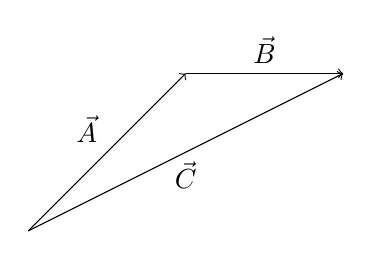
\begin{tikzpicture}
            \draw[black] (0,0) -- (1,1) node[anchor=south east] {$\vec{A}$};
            \draw[black, ->] (1,1) -- (2,2);
            \draw[black] (2,2) -- (3,2) node[anchor=south] {$\vec{B}$};
            \draw[black, ->] (3,2) -- (4,2);
            \draw[black] (0,0) -- (2,1) node[at end, anchor=north ] {$\vec{C}$};
            \draw[black, ->] (2,1) -- (4,2);
        \end{tikzpicture}

    \item \textbf{Subtraction:} $\vec{A} - \vec{B} = \vec{C}$
    
        \begin{tikzpicture}
            \draw[black] (0,0) -- (1,1) node[anchor=south east] {$\vec{C}$};
            \draw[black, ->] (1,1) -- (2,2);
            \draw[black, ->] (4,2) -- (6,2) node[anchor=south] {$\vec{B}$};
            \draw[black, <-] (2,2) -- (3,2) node[anchor=south] {$\vec{-B}$};
            \draw[black] (3,2) -- (4,2);
            \draw[black] (0,0) -- (2,1) node[at end, anchor=north ] {$\vec{A}$};
            \draw[black, ->] (2,1) -- (4,2);
        \end{tikzpicture}

    \item \textbf{Multiplication by a scalar: } $c\vec{A} = \vec{C}$
    \item \textbf{Dot Product: } $\vec{A}.\vec{B} = AB\cos(\theta)$.
        Dot product is a scalar. It is commutative and distributive.
    \item \textbf{Cross Product: } $\vec{A} \times \vec{B} = AB\sin(\theta) \hat{n}$
        where $\hat{n}$ is the unit vector perpendicular to the plane containing $\vec{A}$ and $\vec{B}$.
    \end{itemize}

        Cross product is a vector. It is anti-commutative and distributive.
    \subsection*{Component form of a Vector: }
    A vector $\vec{A}$ can be written as:
    $$\vec{A} = A_x \hat{i} + A_y \hat{j} + A_z \hat{k}$$
    where $\hat{i}, \hat{j}, \hat{k}$ are unit vectors along the $x, y, z$ axes respectively.

    Given that $\vec{A} = A_x \hat{i} + A_y \hat{j} + A_z \hat{k}$ and $\vec{B} = B_x \hat{i} + B_y \hat{j} + B_z \hat{k}$, we can perform the following operations:
    \begin{itemize}
        \item \textbf{Addition (and Subtraction):} $\vec{A} + \vec{B} = (A_x + B_x) \hat{i} + (A_y + B_y) \hat{j} + (A_z + B_z) \hat{k}$
        \item \textbf{Multiplication by a scalar: } $c\vec{A} = cA_x \hat{i} + cA_y \hat{j} + cA_z \hat{k}$, where $c$ is a scalar.
        \item \textbf{Dot Product: } $\vec{A}.\vec{B} = A_xB_x + A_yB_y + A_zB_z$
        \item \textbf{Modulus: } $|\vec{A}| = \sqrt{A_x^2 + A_y^2 + A_z^2}$
        \item \textbf{Cross Product: } $\vec{A} \times \vec{B} = (A_yB_z - A_zB_y) \hat{i} + (A_zB_x - A_xB_z) \hat{j} + (A_xB_y - A_yB_x) \hat{k}$
            This can also be written in a determinant form:
            $$\vec{A} \times \vec{B} = \begin{vmatrix}
                \hat{i} & \hat{j} & \hat{k} \\
                A_x & A_y & A_z \\
                B_x & B_y & B_z
            \end{vmatrix}$$
    \end{itemize}
    \subsection*{Triple Product: }
    \paragraph*{Scalar Triple Product: } $\vec{A}.(\vec{B} \times \vec{C}) = \vec{B}.(\vec{C} \times \vec{A}) = \vec{C}.(\vec{A} \times \vec{B})$
    Geometrically the scalar triple product is the volume of the parallelopiped formed by the three vectors.
    \paragraph*{Vector Triple Product: } $\vec{A} \times (\vec{B} \times \vec{C}) = \vec{B}(\vec{A}.\vec{C}) - \vec{C}(\vec{A}.\vec{B})$
\end{document}